\documentclass[]{IEEEtran}
% some very useful LaTeX packages include:
%\usepackage{cite}      
\usepackage{graphicx}   
\usepackage{subfigure} 
\usepackage{url}       
\usepackage{amsmath}    
\usepackage{caption2}
% Your document starts here!
\begin{document}

% Define document title and author
	\title{Weekly Report}
	\author{Adviser: Prof. Yang Wen \\Student: Cheng Wensheng\\ Period: 2018.9.30-10.7
	}
	\markboth{Visual Information Processing Group}{}
	\maketitle

% Write abstract here
\begin{abstract}
	This week I mainly put my effort on thinking about my paper's idea and reading a new semantic segmentation paper of MIT researchers, which is accepted by SIGGRAPH 2018.
\end{abstract}

% Each section begins with a \section{title} command
\section{Paper reading}
	% \PARstart{}{} creates a tall first letter for this first paragraph
	\PARstart{T}{he} paper's title is \emph{Semantic Soft Segmentation}. In this paper, they approach the problem of dealing with transition parts of image from a spectral segmentation angle and propose a graph structure that embeds texture and color features from the image as well as higher-level semantic information generated by a neural network.

	In summary, the following points show their main contributions:
	\begin{itemize}
		\item They have proposed a method that generates soft segments that correspond to semantically meaningful regions in the image by fusing the high-level information from a neural network with low-level
		image features fully automatically.
		\item They have shown that by carefully
		defining affinities between different regions in the image, the soft segments with the semantic boundaries can be revealed by spectral analysis of the constructed Laplacian matrix. The proposed relaxed sparsification method for the soft segments can generate accurate soft transitions while also providing a sparse set of layers.
		\item They have demonstrated that while semantic segmentation and spectral soft segmentation methods fail to provide layers that are accurate enough for image editing tasks, our soft segments provide
		a convenient intermediate image representation that makes several targeted image editing tasks trivial, which otherwise require the manual labor of a skilled artist.
	\end{itemize}
	
	Fig.~\ref{fig:fw} is the overview of semantic soft segmantatiaon. Fig.~\ref{fig:rt} is the result of foreground objects processing.
	

% Main Part

\newpage
\begin{figure}[!hbt]
%		 Center the figure.
		\vspace{1.7cm}
%		\hspace{50cm}
		\begin{center}
			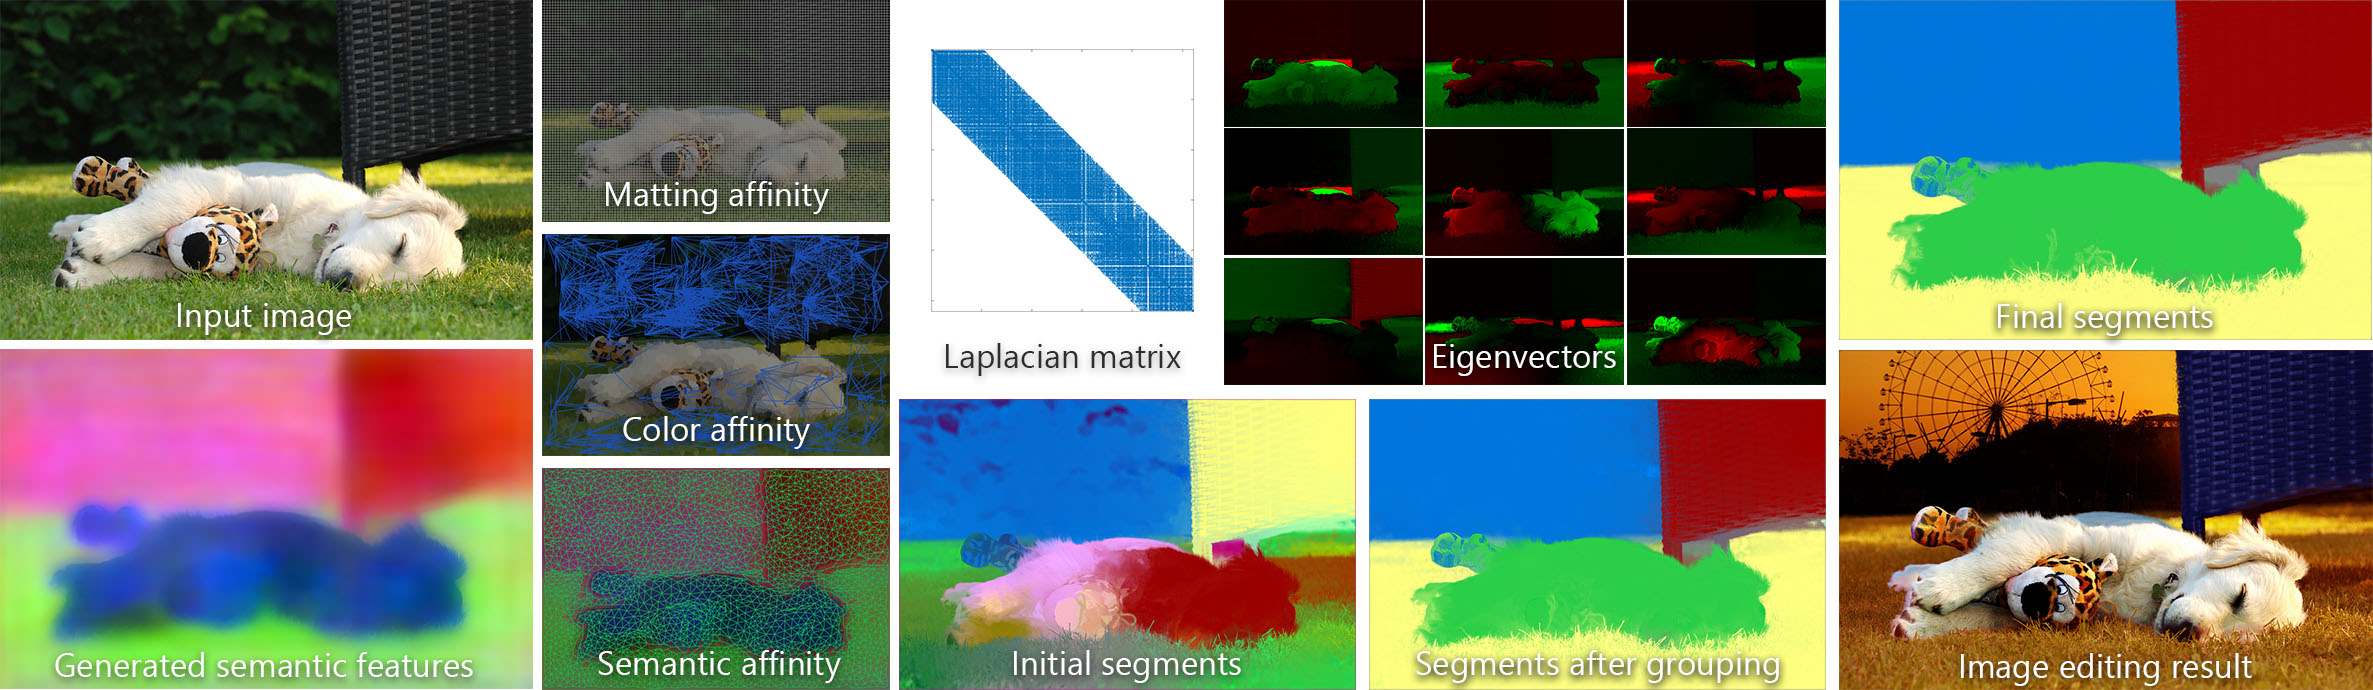
\includegraphics[width=\columnwidth]{fw}
				%		 Create a subtitle for the figure.
			\caption{Pipeline of semantic soft segmantatiaon.}
			\label{fig:fw}
		    \hspace{0.5cm}
			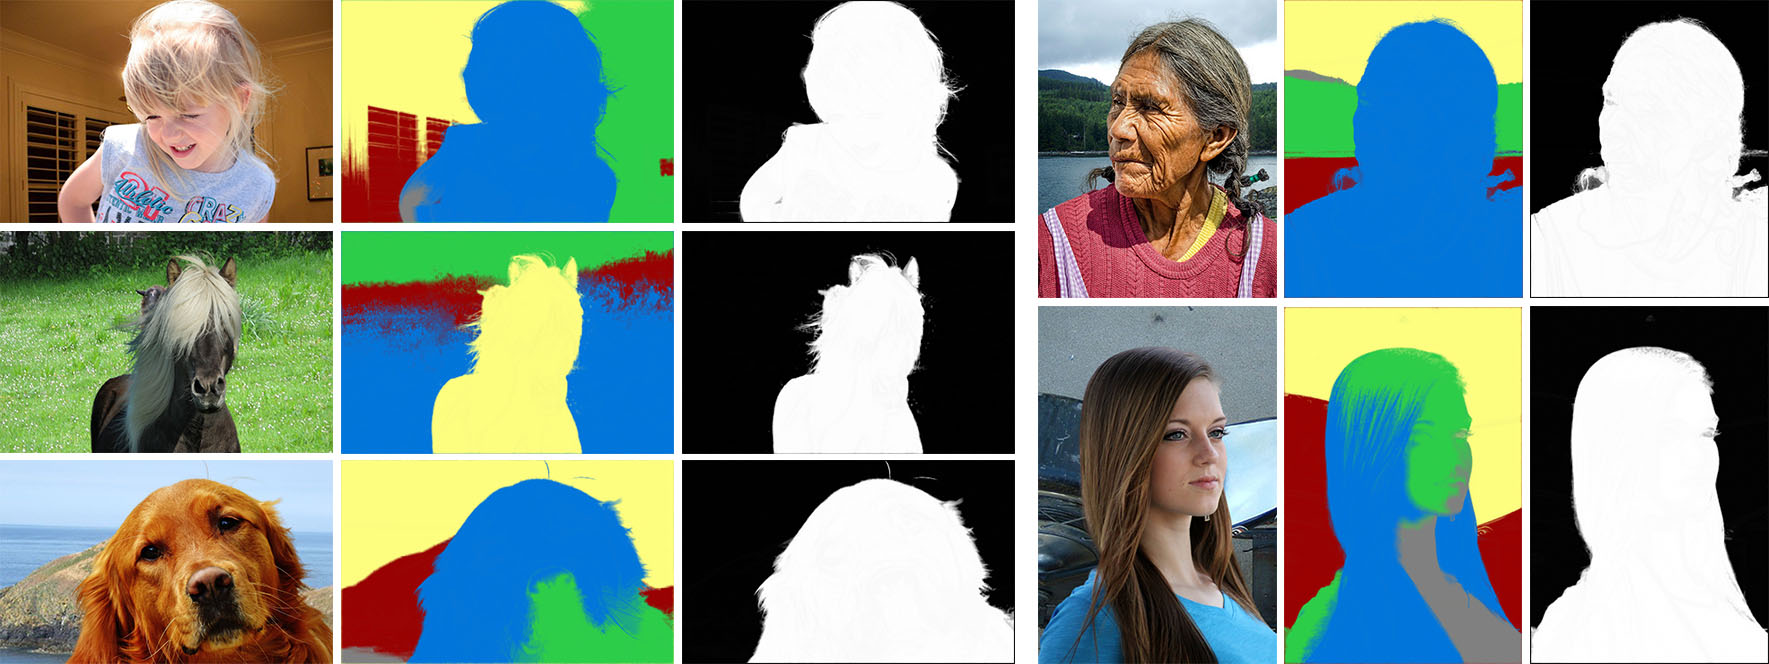
\includegraphics[width=\columnwidth]{rs}
				%Create a subtitle for the figure.
			\caption{Foreground objects processing result.}
			\label{fig:rt}
		\end{center}
	\end{figure}

% Now we need a bibliography:
%\begin{thebibliography}{5}
%
%	%Each item starts with a \bibitem{reference} command and the details thereafter.
%	\bibitem{HOP96} % Transaction paper
%	J.~Hagenauer, E.~Offer, and L.~Papke. Iterative decoding of binary block
%	and convolutional codes. {\em IEEE Trans. Inform. Theory},
%	vol.~42, no.~2, pp.~429–-445, Mar. 1996.
%
%	\bibitem{MJH06} % Conference paper
%	T.~Mayer, H.~Jenkac, and J.~Hagenauer. Turbo base-station cooperation for intercell interference cancellation. {\em IEEE Int. Conf. Commun. (ICC)}, Istanbul, Turkey, pp.~356--361, June 2006.
%
%	\bibitem{Proakis} % Book
%	J.~G.~Proakis. {\em Digital Communications}. McGraw-Hill Book Co.,
%	New York, USA, 3rd edition, 1995.
%
%	\bibitem{talk} % Web document
%	F.~R.~Kschischang. Giving a talk: Guidelines for the Preparation and Presentation of Technical Seminars.
%	\url{http://www.comm.toronto.edu/frank/guide/guide.pdf}.
%
%	\bibitem{5}
%	IEEE Transactions \LaTeX and Microsoft Word Style Files.
%	\url{http://www.ieee.org/web/publications/authors/transjnl/index.html}
%
%\end{thebibliography}

% Your document ends here!
\end{document}